%!TEX root = ../../dissertation.tex
%%%%%%%%%%%%%%%%%%%%%%%%%%%%%%%%%%%%%%%%%%%%%%%%%%%%%%%%%%%%%%%%%%%%%%%%%%%%%%%%
%%%%%%%%%%%%%%%%%%%%%%%%%%%%%%%%%%%%%%%%%%%%%%%%%%%%%%%%%%%%%%%%%%%%%%%%%%%%%%%%
%%%%%%%%%%%%%%%%%%%%%%%%%%%%%%%%%%%%%%%%%%%%%%%%%%%%%%%%%%%%%%%%%%%%%%%%%%%%%%%%
\section{Measurements}
\label{c3:sec:measurements}

%TODO:
%comment on which buffering model is used, both simple models result in smallest buffering time possible, as no overhead waiting is involved

For the YouTube streaming measurements we implemented an automated video downloading and playback simulation software to feed information into the model and evaluate the total stalling time. For this the simple stalling model is used because this results in the shortest possible playback duration in every scenario. Furthermore, we used a network emulation testbed to subject the video streaming to increased loss and latency while fixing the maximum network bandwidth and observe the influence on the QoE.

The first point of interest discovered during the evaluation of the measurements was the information encoded in the URLs pointing to the actual video files (cf. Table \ref{c3:tbl:yturl}) as they hinted on the presence of transmission rate throttling for some videos. However, if one tries to alter or remove the throttling parameters the YouTube server responds to this with a HTTP 403 forbidden error code, meaning that there are further checks in place to ensure this behavior. 

We experienced this hinted throttling for all non-HD (i.e. lower than 720p resolution) videos. The throttling method, which \cite{alcock2011afcyt} also observed, limits the transmission to a rate higher than but correlated to the average media bitrate. The \textit{block-sending} method used for the limiting is rather unusual as it transmits short packet bursts, typically 64 KiB in size, followed by long pauses as seen in Figure \ref{c3:fig:blocktransfer-detail}. Initially, a larger burst is transmitted to allow for some pre-buffering to occur in the client's media player (cf. Fig. \ref{c3:fig:blocktransfer-overall}). This limiting is probably in place to even the load on the caches and to prevent load spikes, yet ensuring that every client receives the necessary data in time for playback.



\begin{figure}[htbp]
% used yt-delay/hPUGNCIozp0_delay_100 2, spyder with matplotlib config patch
	\centering
    	\begin{subfigure}[b]{0.80\textwidth}
                \centering
                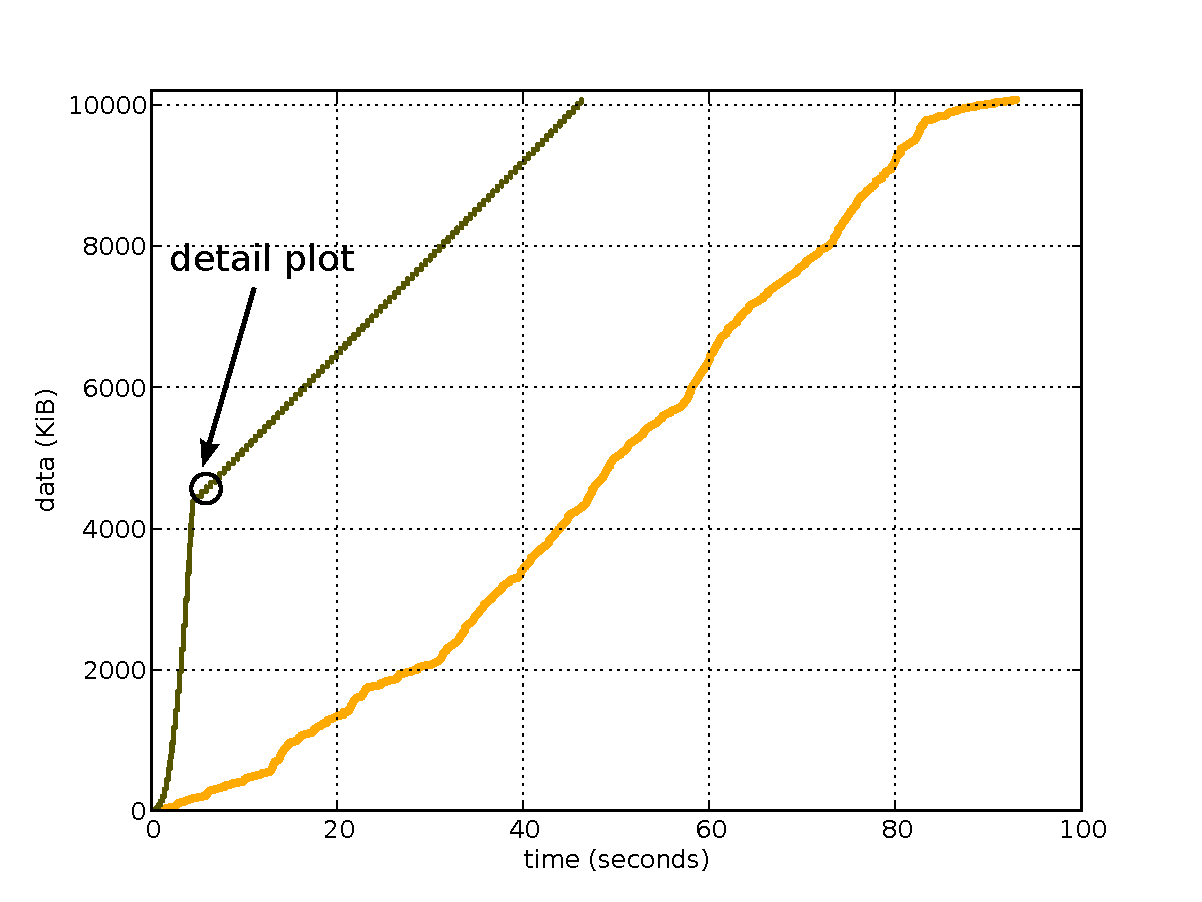
\includegraphics[width=\textwidth]{images/blocktransfer-mod.pdf}
                \caption{Overall graph.}
                \label{c3:fig:blocktransfer-overall}
        \end{subfigure}

    	\begin{subfigure}[b]{0.80\textwidth}
                \centering
                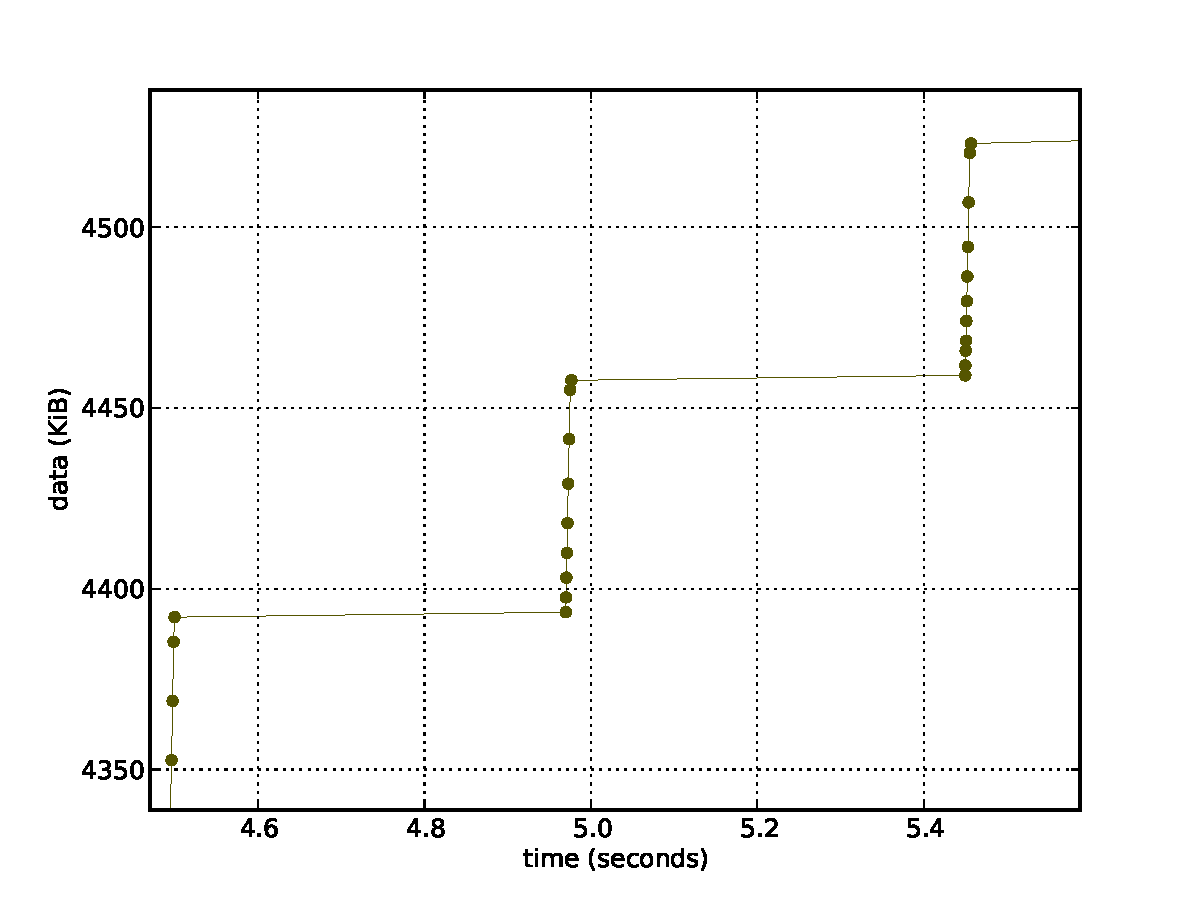
\includegraphics[width=\textwidth]{images/blocktransferdetail.pdf}
                \caption{Detail plot of the rate-limited block-sending phase.}
                \label{c3:fig:blocktransfer-detail}
        \end{subfigure}
\caption{Measurement results for the download and playback of a video.}
\label{c3:fig:blocktransfer}
\end{figure}



\begin{table}[htbp]
% increase table row spacing, adjust to taste
\renewcommand{\arraystretch}{1.3}
\caption{Transmission Related Parameters from YouTube's Video URL Setup}
\label{c3:tbl:yturl}
\centering
\begin{tabu}{|X[l]|X[p]|}
\hline
URL Part & Description \\ \hline
\texttt{v$\alpha$.lscache$\beta$.c.youtube.com} &  Cache server involved in the delivery.\\
\texttt{algorithm=throttle-factor} and \texttt{burst=40} and \texttt{factor=1.25} & Indicates initial burst plus block sending configuration. \\
\texttt{ratebypass=yes} & Parameter to indicate no rate limiting.\\ \hline
\end{tabu}

\end{table}

We performed two measurement series, one with increased packet loss, the other one adding latency to the path. For each value of loss and latency a mean total stalling time was calculated out of five separate experiments to eliminate temporal and network load influences. Additionally, standard deviations are shown in the resulting graphs of Figure \ref{c3:fig:seriesgraphs}. We clearly notice very large deviations in some experiments. Some of these can be explained by connection timeouts and later resumption of the streaming. Furthermore, an exponential regression line shows the trend of the total stalling times in the experiments.


Figure \ref{c3:fig:delayseries} displays the results of of the latency measurement series with up to five seconds of additional delay. In the worst case the stalling time increases to about 50 seconds. In mobile scenarios latencies of up to 2 seconds can be expected, which would, according to our measurements, result in a maximum mean stalling time of 15 seconds for a 90 second video, which could very well be bearable for YouTube users.

There are several factors that could contribute to the increase in stalling time in the latency experiments. 
TCP, in its simplest form, increases the congestion window based on the Round Trip Time (RTT), making it highly dependent on this connection parameter. Newer congestion avoidance algorithms, e.g. the CUBIC algorithm used in Linux \cite{ha2008cubic}, however reduce this dependence on the RTT.
Another influencing factor might be YouTube's block sending mechanism, which, according to \cite{alcock2011afcyt}, may negatively interact with congestion control algorithms. The impact of packet loss on stalling is much higher than that of latency in our measurements. Yet, due to TCP's reliable transmissions, loss only causes increased packet retransmissions, and, thus, acts as a source of burst delay which negatively impacts the overall throughput.

Figure \ref{c3:fig:lossseries} shows the series of loss experiments. While the 6\% packet loss and below has an almost negligible influence on the stalling time anything above this value will probably not achieve good user experience at all. Interesting to note is the rather sudden increase in stalling time when there is more than 6\% loss added. This could again hints to the transport protocol's reliable transport feature, which catches all the occurring losses, through timeouts or gaps in the sequence numbers. However, the detection and retransmission takes some time, which is reflected in the increased stalling time.





% TODO: Mobile video delivery with HTTP \cite{ma2011mobile}
% reasoning for "HTTP pacing" and segmented delivery

\begin{figure}[htbp]
% yt-delay-allBW.ods, graphik aus LibreOffice Calc, OLE in LibreOffice Draw, font sizes min 11pt, Page Margins passen (18,2 x 10,3), als PDF exportiert.
% new method: extra libreoffice calc page, scaled to fit on one page, pdf export, cut with acrobat
	\centering
    	\begin{subfigure}[b]{1.0\textwidth}
                \centering
                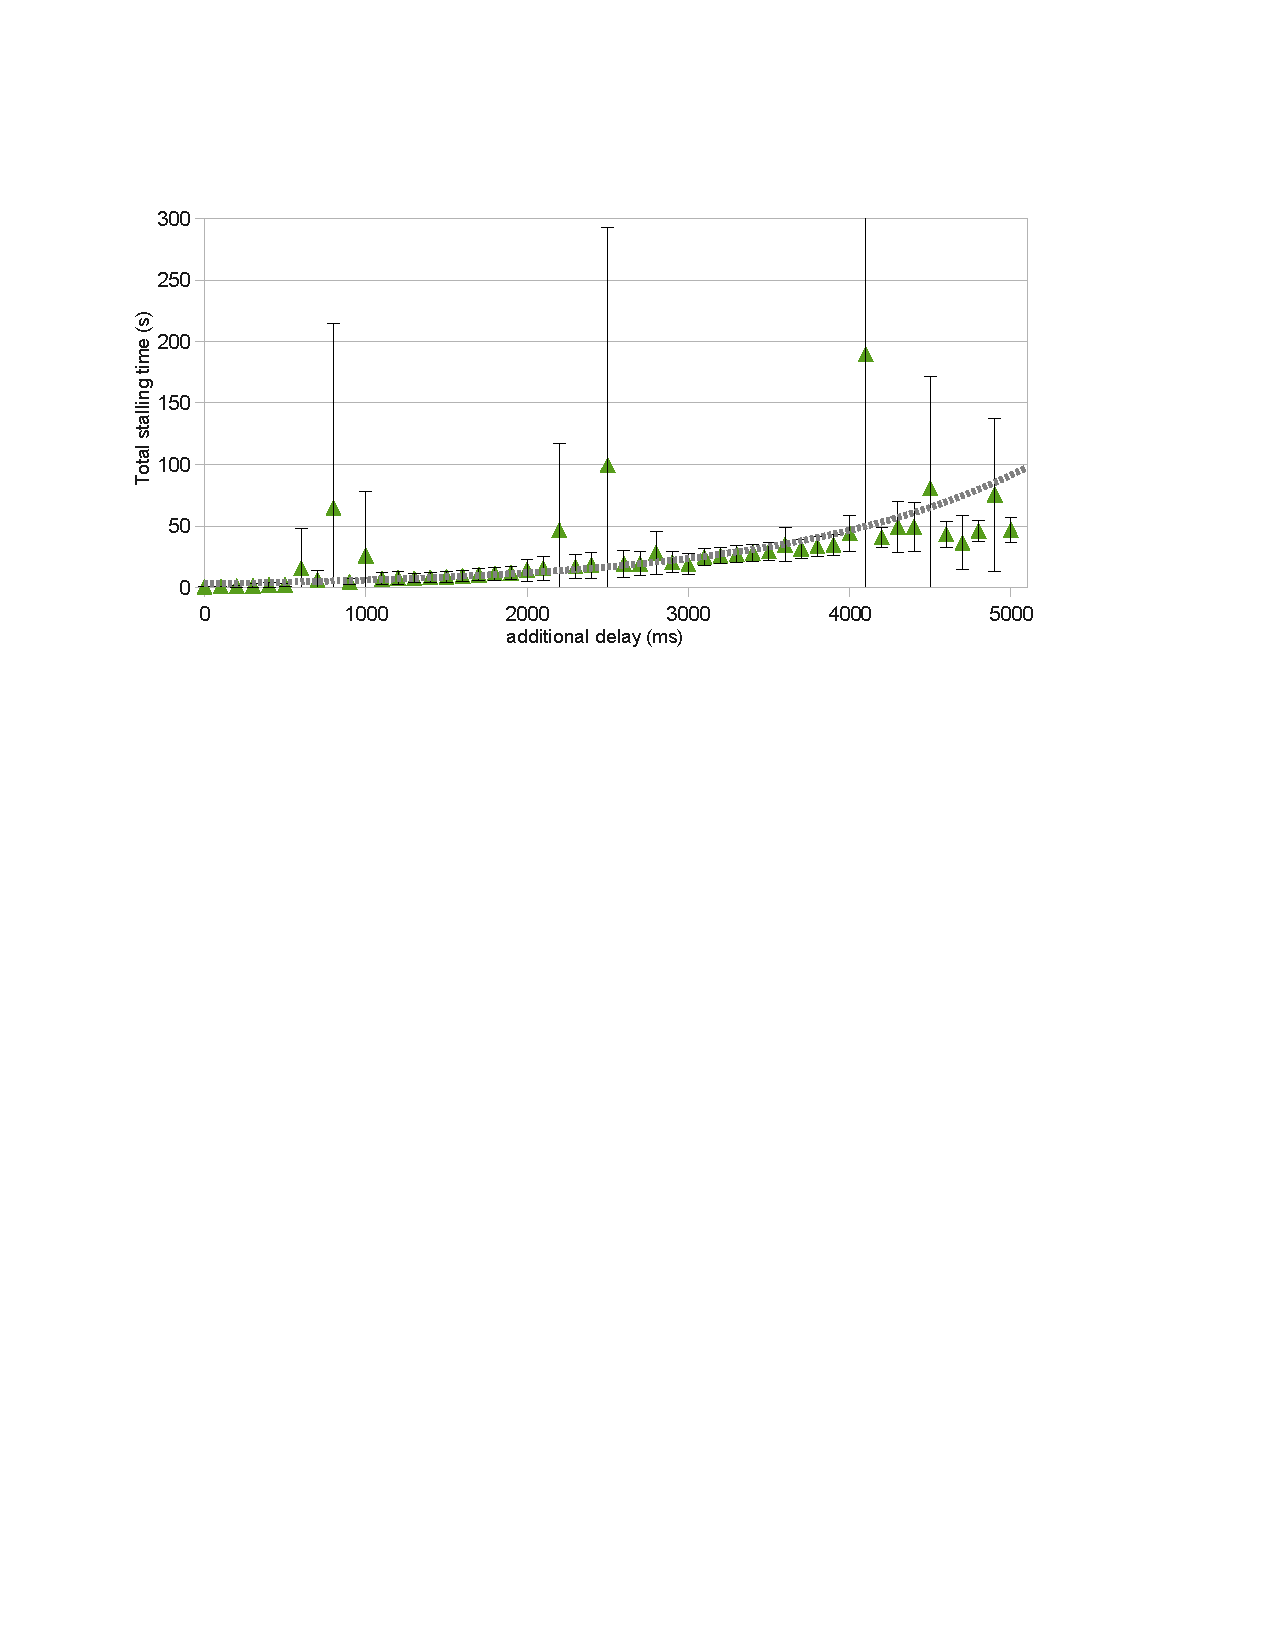
\includegraphics[width=\textwidth]{images/delay.pdf}
                \caption{Latency Graph.}
                \label{c3:fig:delayseries}
        \end{subfigure}

    	\begin{subfigure}[b]{1.00\textwidth}
                \centering
                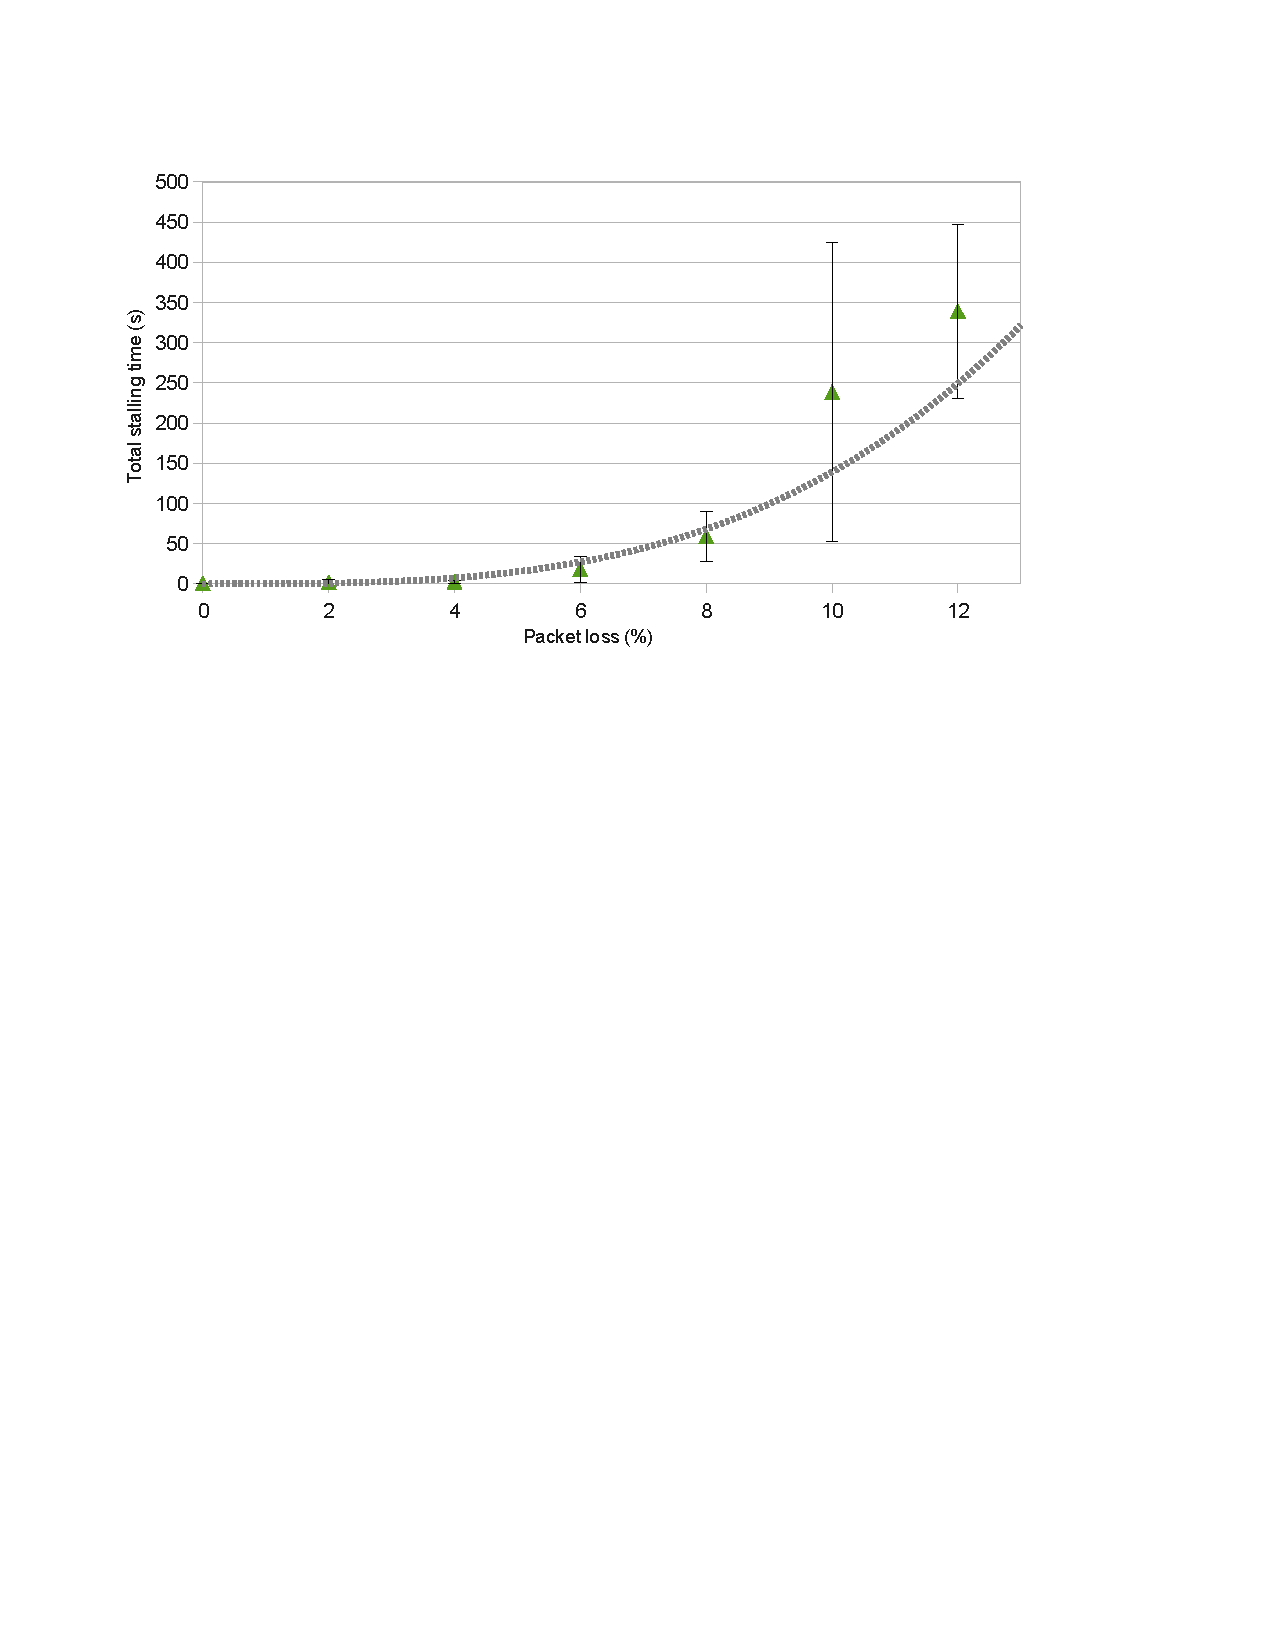
\includegraphics[width=\textwidth]{images/loss.pdf}
                \caption{Loss Graph.}
                \label{c3:fig:lossseries}
        \end{subfigure}
\caption{Total buffering time and exponential trend for degraded network parameter scenarios.}
\label{c3:fig:seriesgraphs}
\end{figure}




%%%%%%%%%%%%%%%%%%%%%%%%%%%%%%%%%%%%%%%%%%%%%%%%%%%%%%%%%%%%%%%%%%%%%%%%%%%%%%%%
\subsection{Testbed Architecture}

Testing and comparing new protocols is a complex and time-consuming undertaking if traditional evaluation approaches such as analytical source-traffic models are employed. For today's fast-paced development of streaming protocols, faster evaluation methods are needed. A testing environment must be simple and sufficiently flexible to allow its application on and adaption to current and future protocols, services, network structures, and associated parameter spaces. 
% This also demands to take a generic approach that does not rely on specific implementations. 
At the same time, it must be able to answer specific questions about  protocols, applications, and network setups. Finally, the results yielded from analyzing and evaluating a streaming service should be user-oriented, i.e. provide a foundation of data that can be fed into the calculation of a Quality of Experience (QoE) model. We believe our proposed testbed, the architecture of which will be explained in the following, meets these requirements.

%In the following sections, we first describe the methodology and then present exemplary evaluations to show how this approach can be used to evaluate real world streaming scenarios under configurable network conditions. 
% Through configuration, one may evaluate the influence of network parameters, states, and topologies on the multimedia stream, e.g. parallel bearers with different quality settings, cross traffic, or stream-support middleboxes.


Figure \ref{c3:fig:testbed} depicts the evaluation testbed. % To enable rapid comparison of network quality of service against application behaviors we employ a two-step process. 
Conceptually, it replicates the actual steps a user would perform to consume a media stream on a playback device. Through appropriate configuration different scenarios can be modeled, e.g. network conditions, behavior and specifics of the user device.
 
 
\begin{figure}[htbp]
	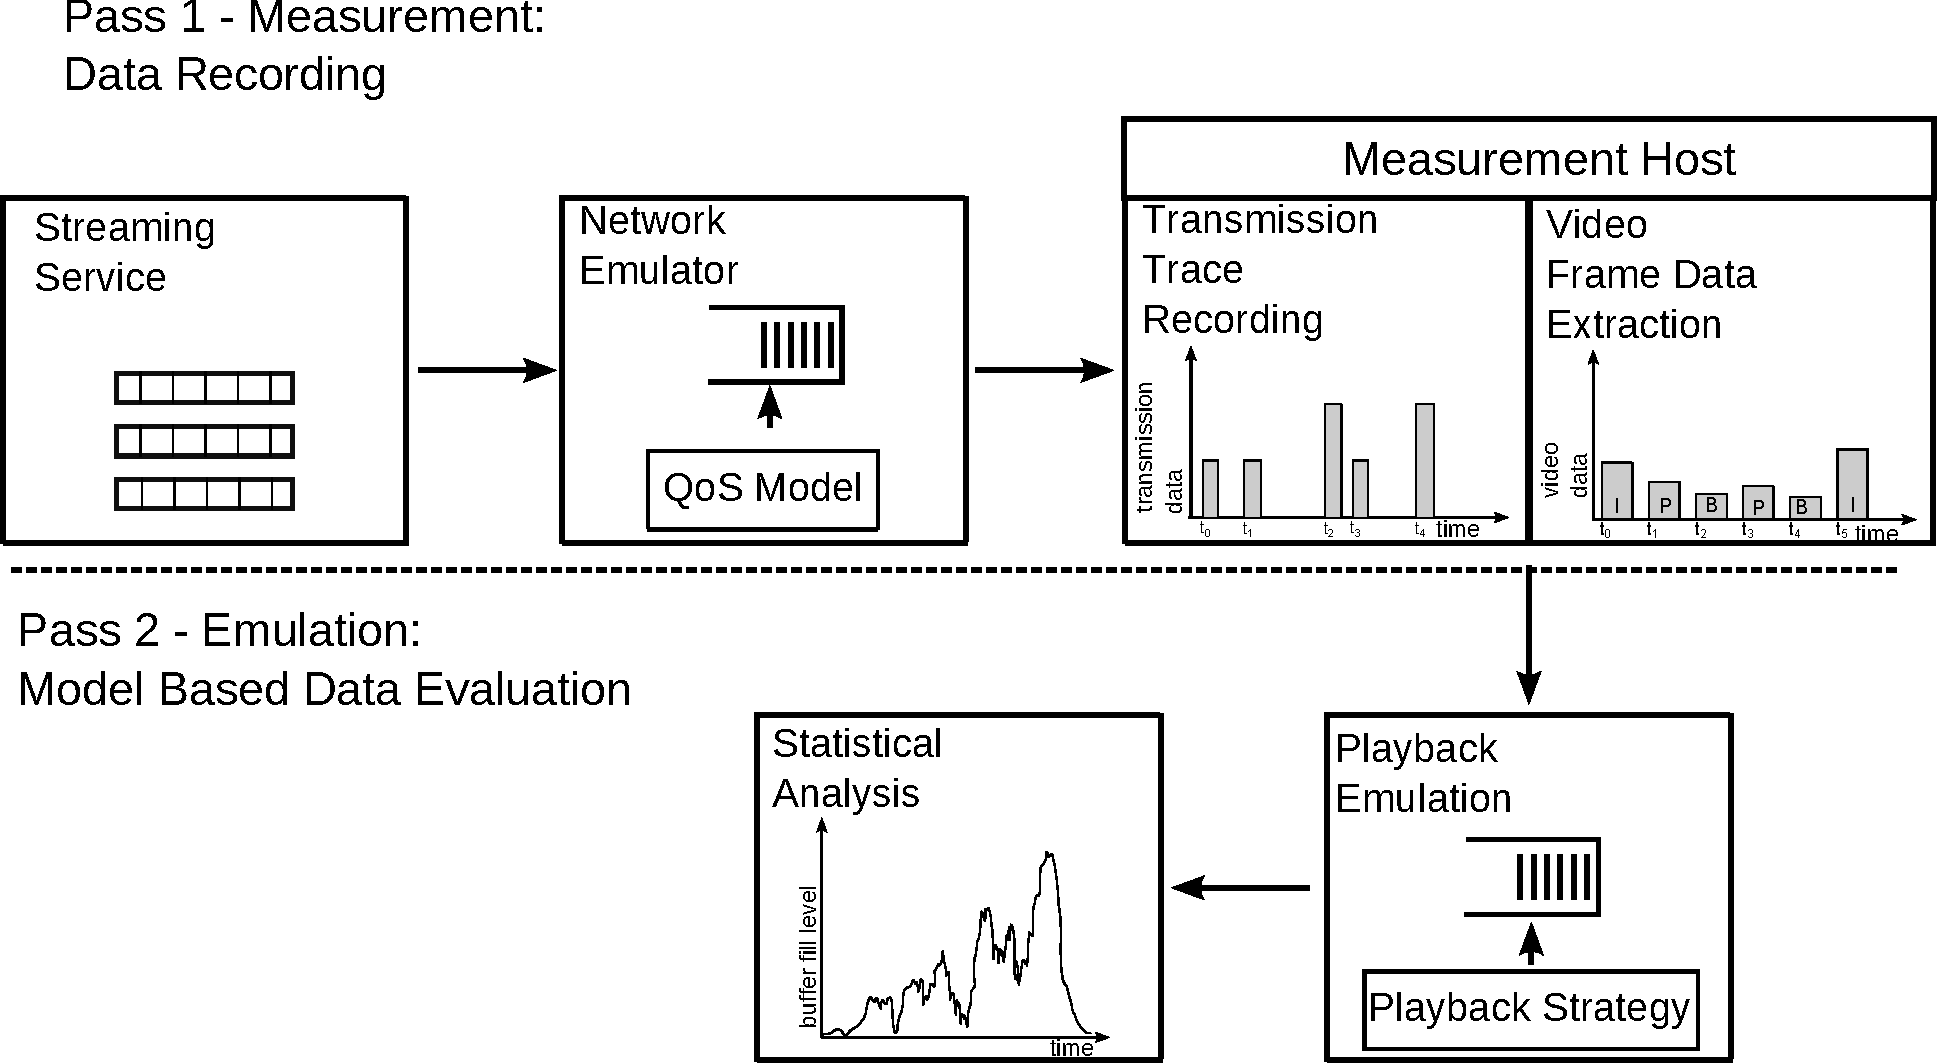
\includegraphics[width=\textwidth]{images/measurement-model.pdf}
	\caption{Testbed Schematic.}
	\label{c3:fig:testbed}
\end{figure}

In the first pass of the process, the stream data is transmitted from a server to the client. The server can either be an actual streaming service on the Internet, or a local server (to eliminate the unpredictable impact of the Internet connection). The traffic is directed through a network emulation node capable of altering the network QoS parameters, i.e. latency, jitter, and packet loss. The parameters could also be set according to stochastic models derived from actual network traces. 
%Therefore, almost any kind of access network conditions can be modeled. 
%Of particular interest are mobile radio behaviors and core network architectures. An example would be to compare guaranteed bit rate (GBR) with best-effort PDP contexts to assess the impact of QoS parameters on the stream quality.

The measurement host downloads and records the video stream as a network trace. For HTTP streaming, it issues a single HTTP \texttt{GET} request on the video file, and then maintains the TCP connection until the file has fully arrived. A trace should at least contain the sizes and timestamps of every incoming packet. More detailed traces can be used to scrutinize other layers of the connection, e.g. the dynamics of TCP receive window size. The packet trace is then decoded using the popular open source \texttt{ffmpeg} suite, yielding another set of traces consisting of video frame sizes and playout timestamps.

In the second pass, these two traces are then used to feed the playback models described before. The playback emulation process combines the transmission and video frame traces to calculate the playback buffer fill level for every point in time during the playback. It then generates statistics about user-perceivable artifacts such as playback stalls that would occur during the playback. These statistics can then be compared to the results of other models and network QoS.

% For simple HTTP streaming, there is no feedback from the client to the server that would result in adaptions of the stream (``rate control''). Therefore, recording the packet trace and simulating playback are decoupled, as the latter cannot influence the former. As such, the testbed can test and compare several playback models on the same recorded network trace. This enables fast and efficient comparison of non-feedback protocols subject to the same network conditions.



%%%%%%%%%%%%%%%%%%%%%%%%%%%%%%%%%%%%%%%%%%%%%%%%%%%%%%%%%%%%%%%%%%%%%%%%%%%%%%%%%%%%%%%%%%%%%%%%%%%%
\subsection{Evaluation}
\label{sec:evaluations}

The results presented here show some of the capabilities in comparing play network conditions based on playback models. We compare how the four playback models introduced previously fare against each other in a measurement series featuring  emulated transmission latency and packet loss . At the same time, we acknowledge that other specific questions are not touched in this first set of experiments, e.g. the inclusion of a mobile network or handset, or RTP-based streams.

The video used in our measurements was streamed from the YouTube web site. This provides a realistic base for all the experiments. Note that YouTube also employs its own form of application layer flow control in addition to TCP's \cite{alcock2011application}. % The influence of the access bandwidth can mostly be neglected with this mechanism as long as the limit is well above the video bitrate, which was the case here.
Details on the streamed video are available in Table \ref{c3:tbl:videoparams}.

\begin{table}[htbp]
	\centering
	\caption{Test Video Parameters}
	\label{c3:tbl:videoparams}
	\begin{tabu}{|l|X[r]|}
    \hline
    Parameter & Value \\ \hline
	Video Duration	& 01:32.536 minutes \\
	Size & 9.61 MiB \\
	Framerate & 23.976/s \\
	Average Video Bitrate & 871 Kbps \\
	Codec & AVC+AAC \\ \hline
	\end{tabu}
\end{table}

For the loss experiment series, the network emulator was configured to drop a certain percentage of packets based on a normal distribution on both the uplink and the downlink direction. There was no loss correlation involved, the existence of which one would expect, e.g., in wireless networks. One streaming run for every two percentage points of additional loss up to 14\% was conducted.
In the latency series, the emulator delayed the delivery of every packet for a set constant amount of time. Half of the total amount is added to the uplink the other half to the downlink. One experiment was conducted for every 100ms of additional delay, up to a total of 5000ms.

After the traces were recorded, every playback model was applied to all runs. For every model, two data points were computed. First, the total stalling time was calculated. This is the time the player keeps buffering and not playing the video, including the initial start delay. To attain results comparable to the other measurements, the stalling time is calculated relative to the total video length instead of an absolute value. The second resulting value is the number of times the video stops playing including the initial delay, i.e. the stalling frequency. Both of them are an indicator how well the playback mechanism can cope with the currently emulated network setup. They could for example be used to either check if a modification to a network has a noticeable impact on streaming experience, or to find an optimized player behavior for a given network.

All models will generally work very similar in good network conditions. If sufficient bandwidth is available, they will play videos with almost no delay and  intermediate buffering. If, however, the achievable TCP goodput is close to the average video bitrate, the buffer may be strained by short deviations from the average rates. %TCP goodput can also be severely limited by high latency and loss. Many TCP congestion control algorithms depend on the round trip time. If the RTT is high, the congestion window will increase much slower.

High latency can also trigger TCP timeouts and retransmissions, and in turn decrease the congestion window, further impacting the goodput. The latency measurements are depicted in Figure \ref{c3:fig:eval-latency}. The stalling time increases with the additional latency. The Initial Start Delay model provides the best possible result in terms of pure stalling time. On the other hand, Figure \ref{c3:fig:eval-latency-numstalls} shows the Stalling model provides always the worst result for the number of stalls. Any other model will lie beyond that line. The Flash and HTML5 models both run in just a few buffering events which however tend to increase in length with rising latency. Attributed to the simple and optimistic assumption of the Flash model, stalling time is usually lower than with HTML5, at the cost of slightly more buffering events.
 

\begin{figure}[htbp]
	\centering
    	\begin{subfigure}[htbb]{0.9\textwidth}
            \centering
            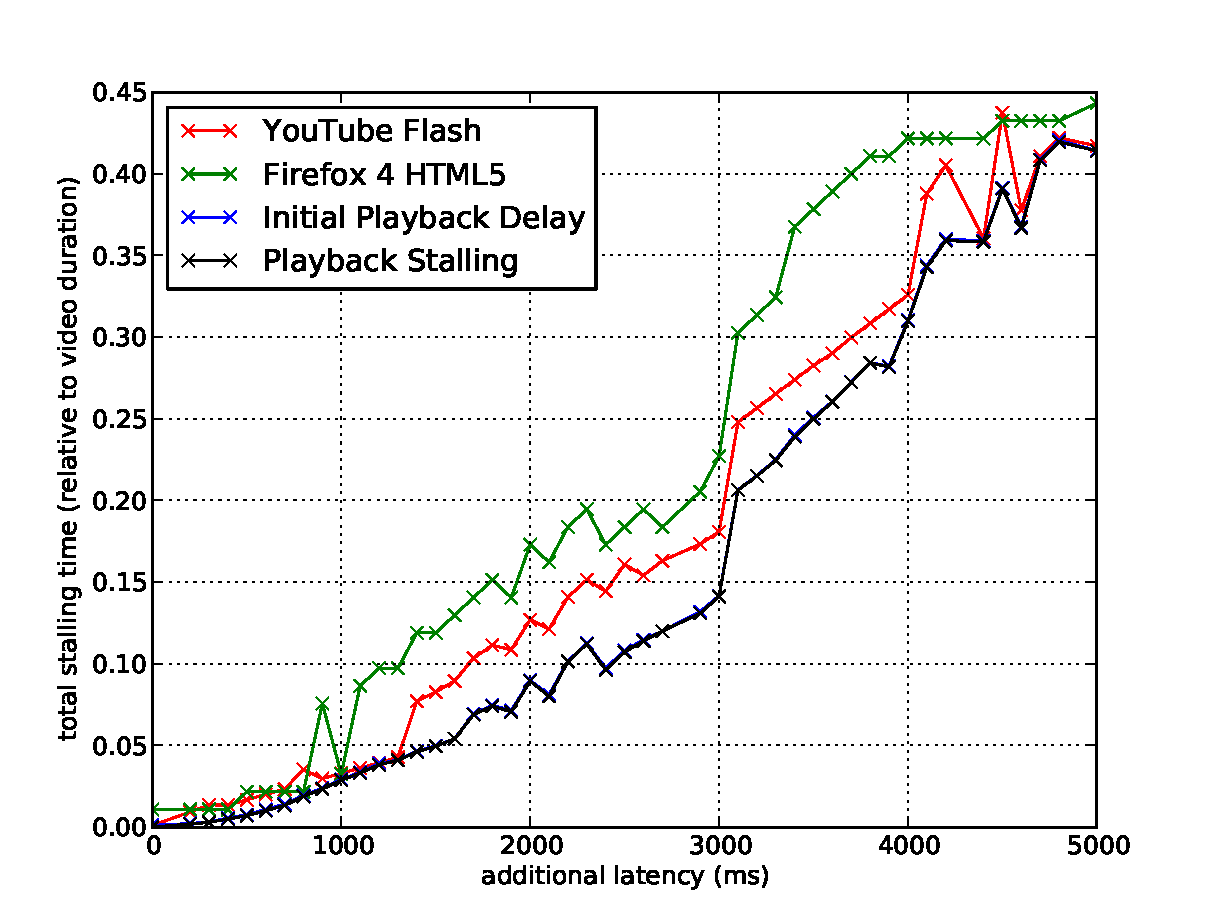
\includegraphics[width=\textwidth]{images/eval-latency-stallingtime.pdf}
            \caption{Total stalling time.}
            \label{c3:fig:eval-latency-stallingtime}
        \end{subfigure}

    	\begin{subfigure}[htbp]{0.9\textwidth}
            \centering
            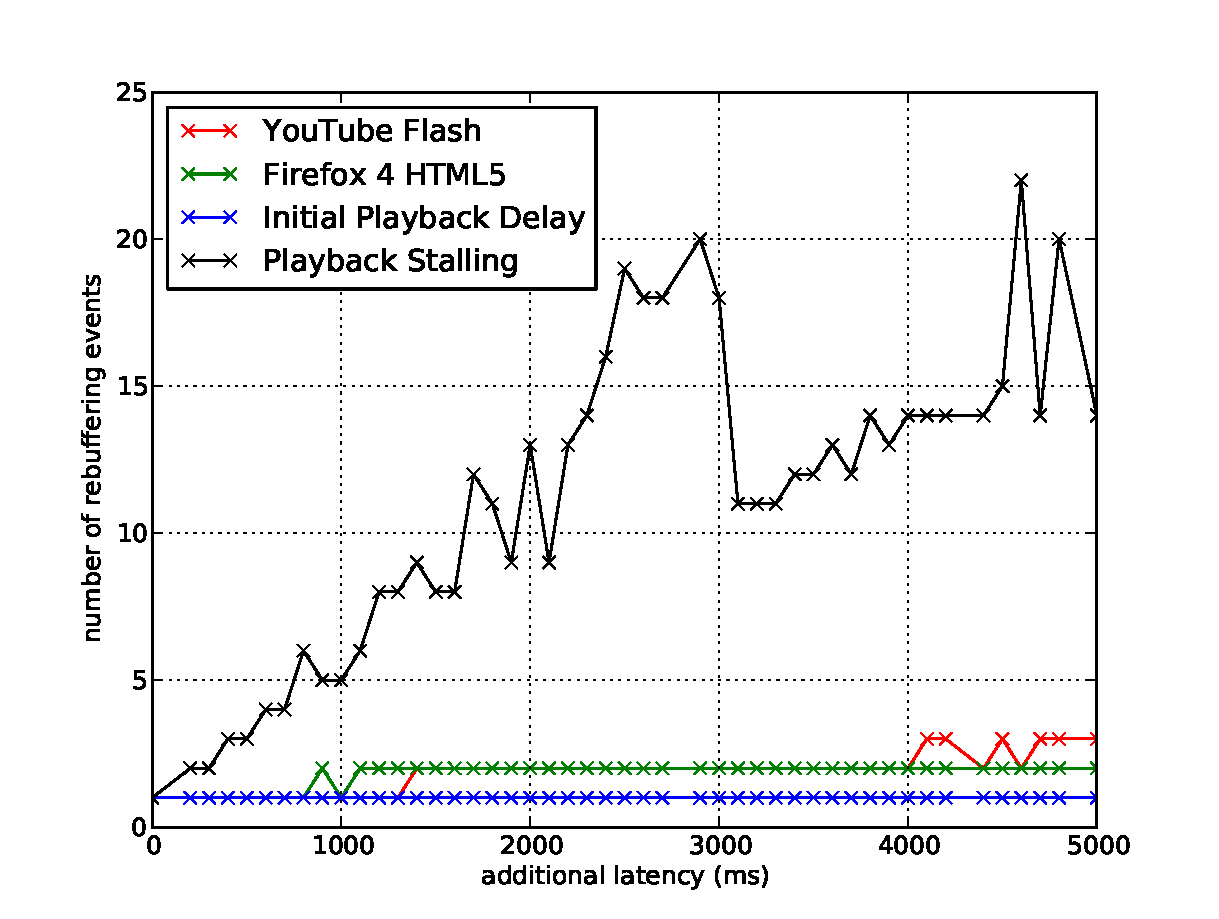
\includegraphics[width=\textwidth]{images/eval-latency-frequency.pdf}
            \caption{Number of stalls.}
            \label{c3:fig:eval-latency-numstalls}
        \end{subfigure}
	\caption{Playback model observations on additional latency.}
	\label{c3:fig:eval-latency}
\end{figure}


TCP goodput is even more severely affected by packet loss. A lost packet results in a duplicate acknowledgement, retransmissions, and a decrease of the congestion window. The problem gets worse if also the ACKs are lost and the connection stalls on missing old segments without which the playback cannot proceed. Figure \ref{c3:fig:eval-loss} shows some exemplary measurements for a loss scenario. While additional packet losses of up to four percent seem to have no noticeable impact on streaming quality, the total stalling time suffers a large increase for any model as seen in Fig. \ref{c3:fig:eval-loss-stallingtime} rendering any streaming attempts practically unusable. Figure \ref{c3:fig:eval-loss-numstalls} shows the extremity of the Stalling model compared to other models reaching a number orders of magnitude larger than any other model.
As a result, when planning a network for streaming applications, the maximum loss should be kept below the noticed mark to achieve reasonable streaming quality. 


\begin{figure}[htbp]
% used yt-delay/hPUGNCIozp0_delay_100 2, spyder with matplotlib config patch
	\centering
    	\begin{subfigure}[htbp]{0.9\textwidth}
            \centering
            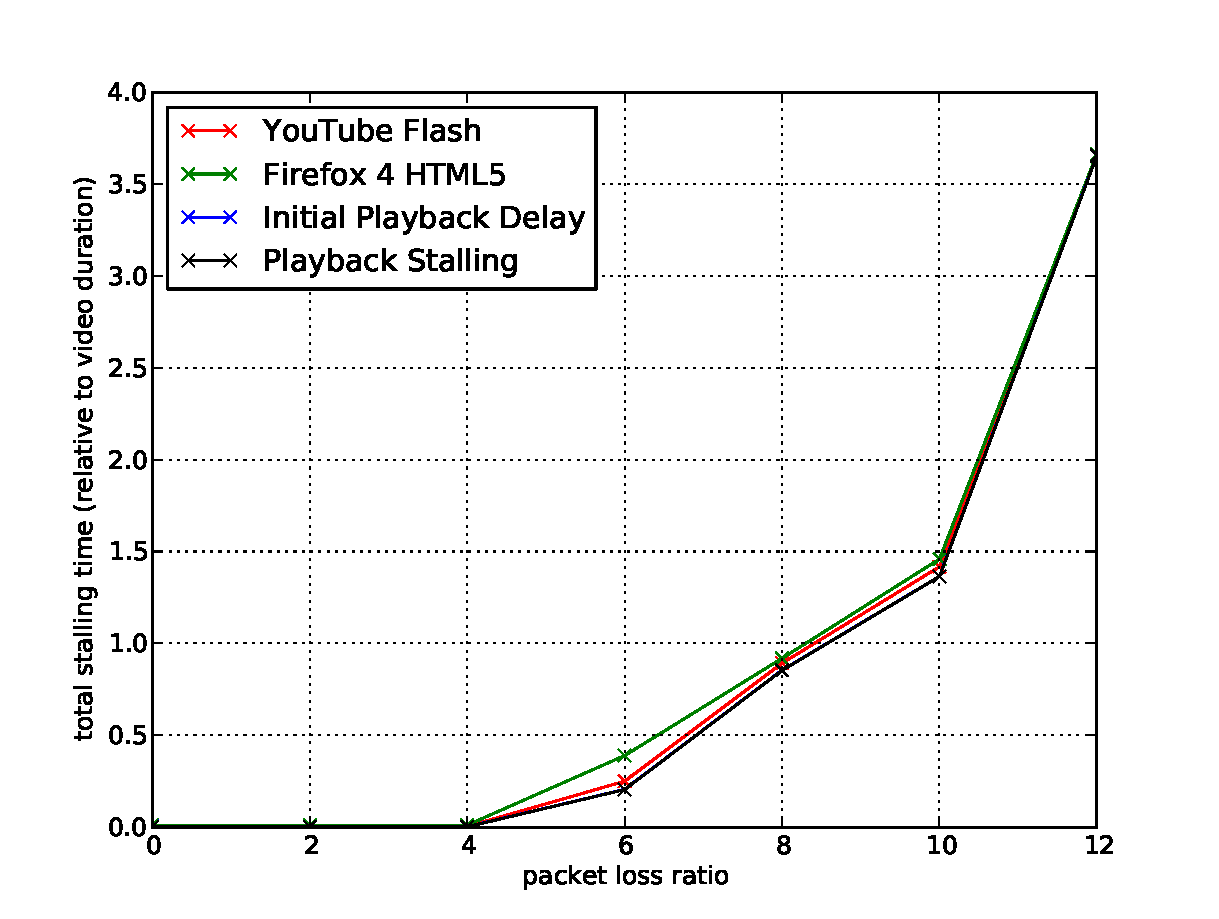
\includegraphics[width=\textwidth]{images/eval-loss4mb-stallingtime.pdf}
            \caption{Total stalling time.}
            \label{c3:fig:eval-loss-stallingtime}
        \end{subfigure}

    	\begin{subfigure}[htbp]{0.9\textwidth}
            \centering
            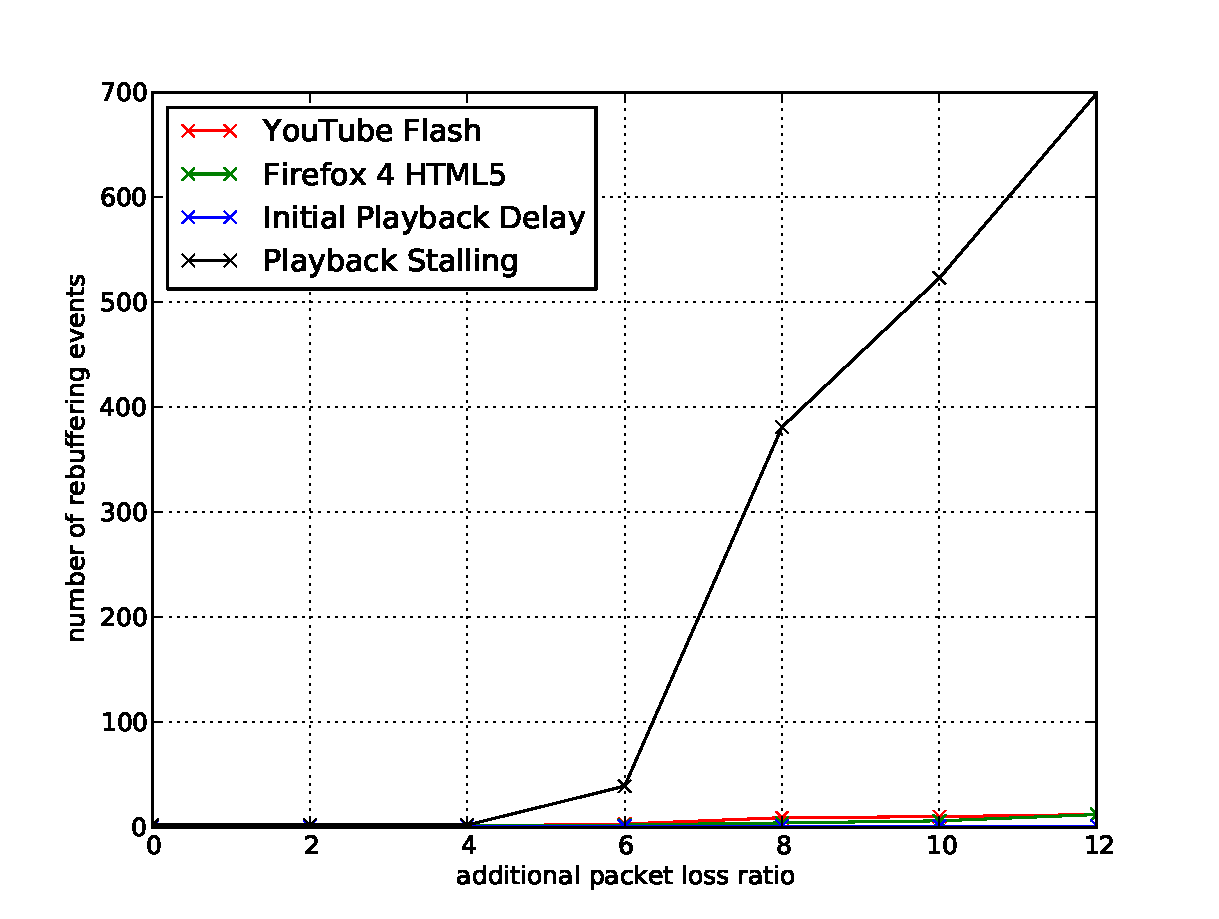
\includegraphics[width=\textwidth]{images/eval-loss4mb-frequency.pdf}
            \caption{Number of stalls.}
            \label{c3:fig:eval-loss-numstalls}
        \end{subfigure}
	\caption{Playback model observations on additional packet loss.}
	\label{c3:fig:eval-loss}
\end{figure}
 
Through these to exemplary experiments, we tried to show that network QoS parameters have a direct measurable impact on the application layer, namely on HTTP streaming quality. While the models scale rather well with latency, any HTTP streaming is almost impossible with high packet loss values.
Comparing the presented playback models, we conclude that every model represents a trade-off between several parameters, e.g. as measured here, the number and length of stalls. With the knowledge gained from the experiments, playback models could be tailor-made to best suit certain conditions and user requirements. 

%The behavior of the existing models is summarized in the table as follows:

%\begin{table}
%\centering
%\begin{tabular}{l|p{1cm}|p{1cm}|p{1cm}|p{1cm}}
% & \textbf{Start Delay} & \textbf{Stalling} & \textbf{YouTube Flash} & \textbf{Firefox HTML5} \\ \hline \hline
%\textit{\# of stalls} & min & max & med & low \\ \hline
%\textit{Duration of stalls} & min & min & med & high \\ \hline
%\end{tabular}
%\caption{Stalling Trade-Offs of the Playback Models}
%\label{tbl:modeleval}
%\end{table}

	
